\documentclass{ximera}

\author{Bart Snapp}

\title{Working with git}

\begin{document}
\pdfOnly{\onecolumn}
\begin{abstract}
    We introduce you to \texttt{git}, and help you make changes on your own.
\end{abstract}
\maketitle
Once you've deployed our content in a GitHub codespace, you'll surely want to
change it and  make it your own.
\begin{image}
    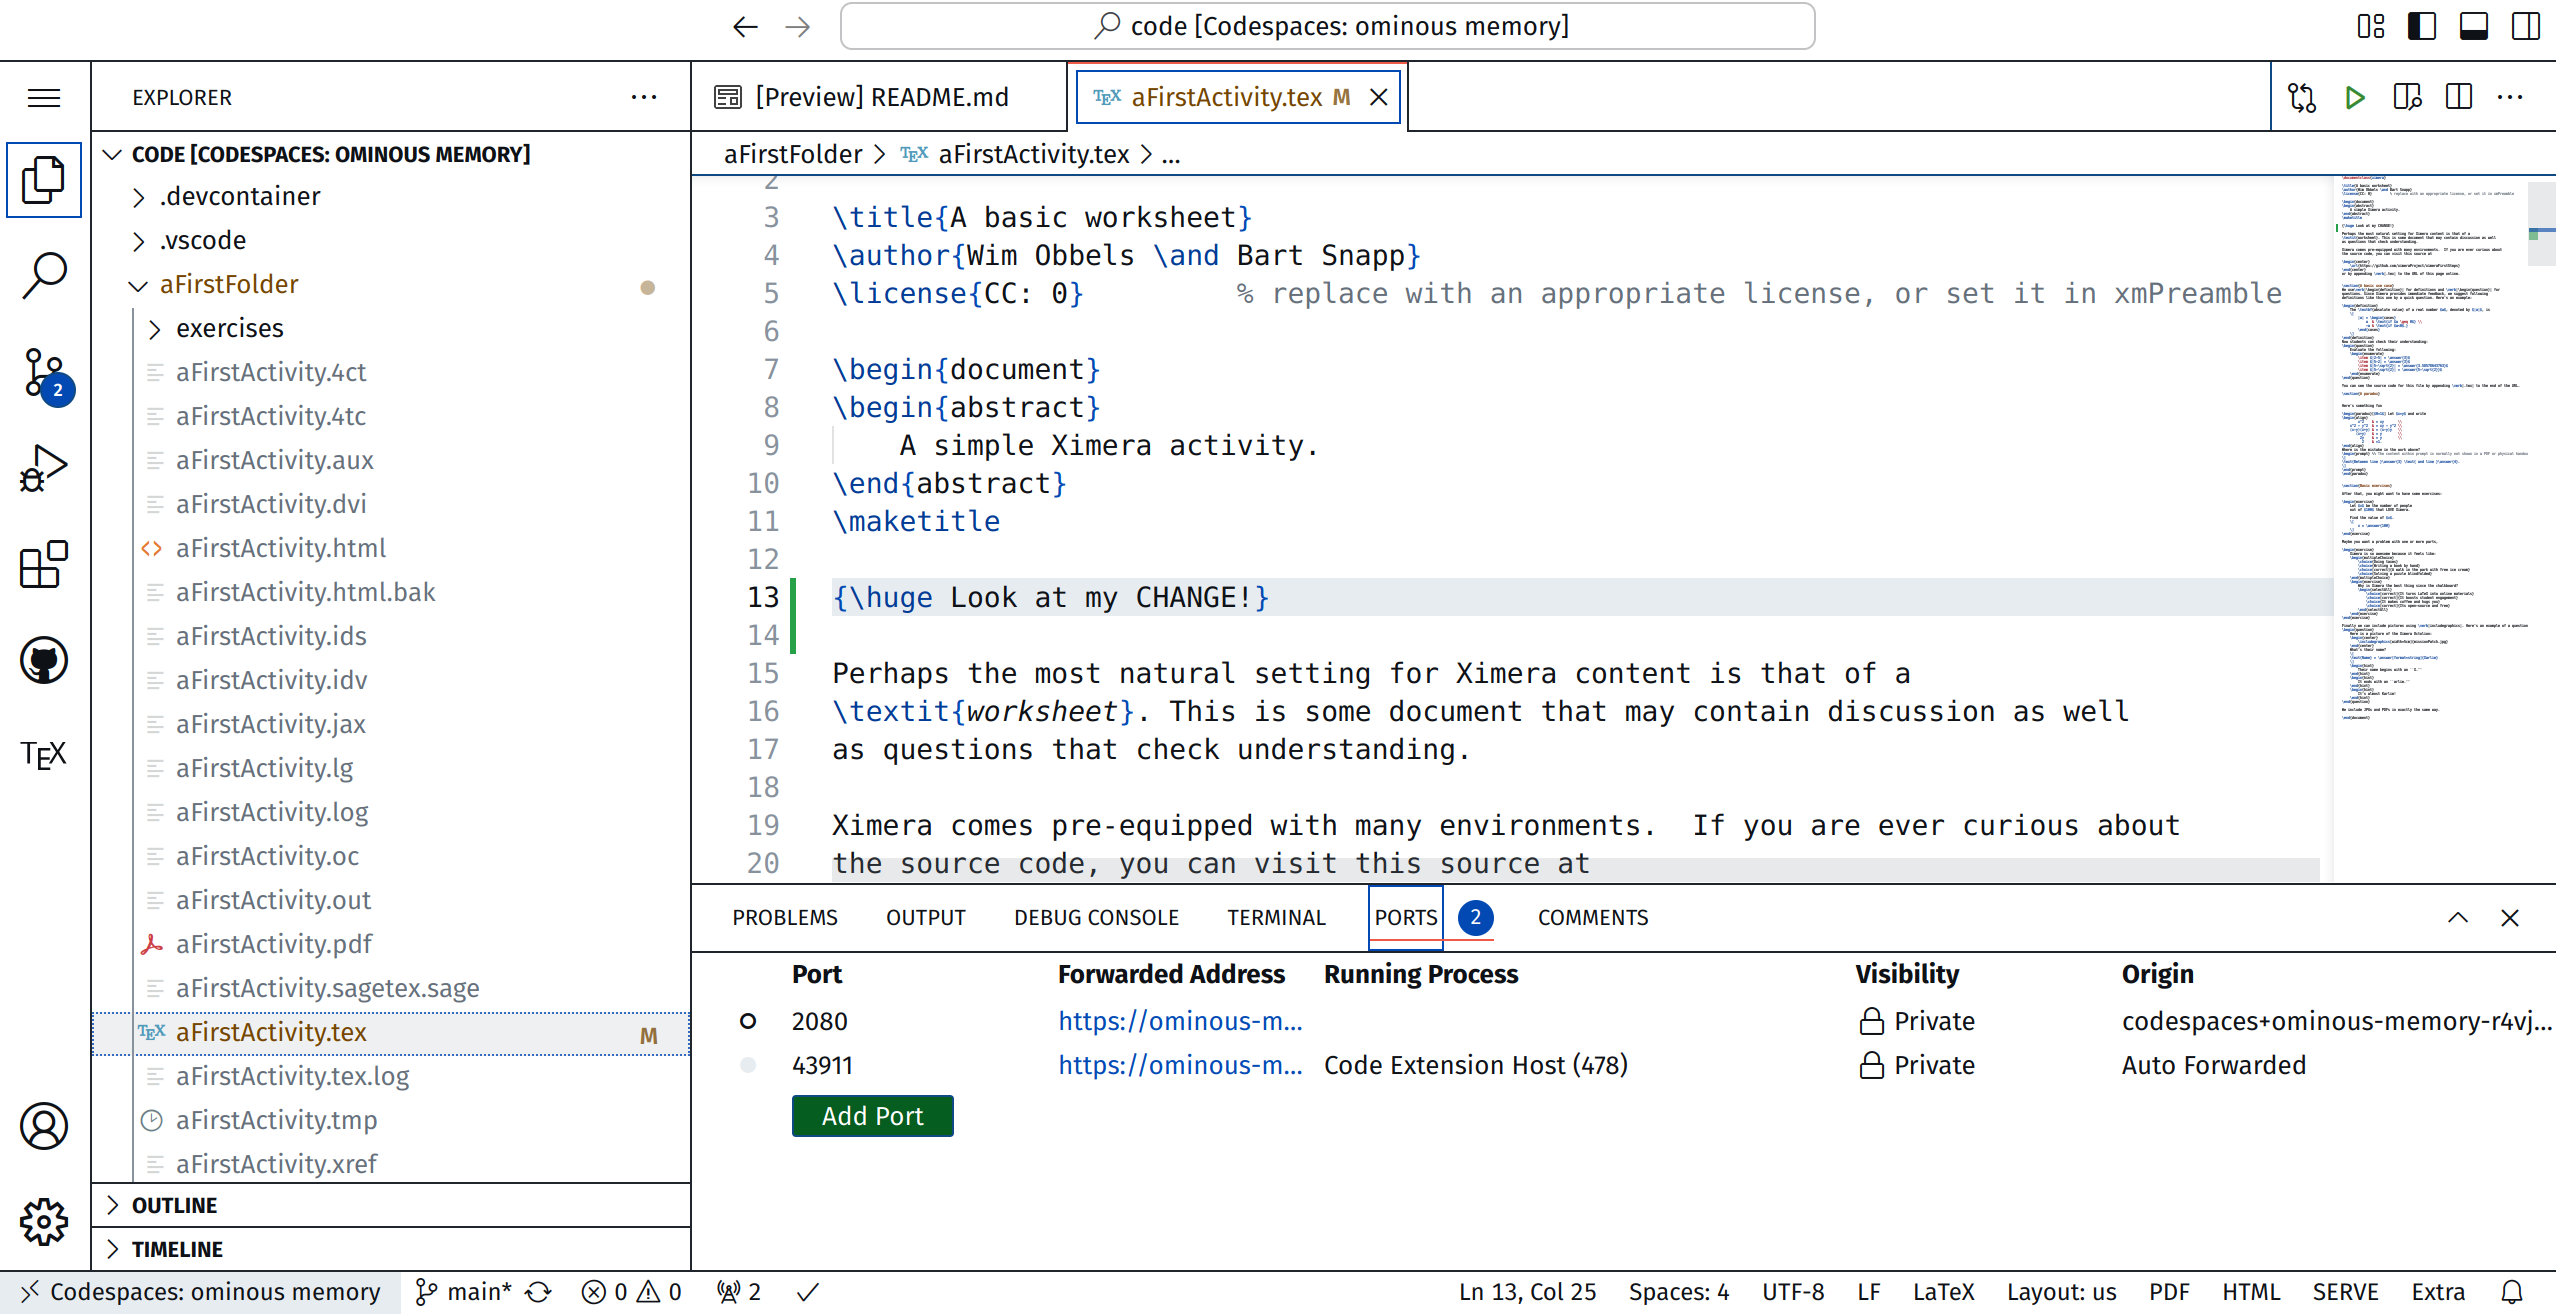
\includegraphics[width=.7\textwidth]{xfsChange}
\end{image}
\pdfOnly{\begin{multicols}{2}}
    Within codespace, you are running VS Code, a
    full-fledged text editor. You can make changes directly there. Our files
    are on
    the left, and are revealed by the ``pages'' icon.
    Here, I've opened the folder \verb!aFirstFolder!, and then the document
    \verb!aFirstActivity.tex!. I made a change in the middle of the screen.

    At this point, you may push ``SERVE'' and see the results of your change;
    however, \textbf{these changes were made only in your temporary codespace},
    a
    virtual
    computer, lost in the cloud. To make these changes to your actual GitHub
    repository, you need to ``Sync'' them back.
\pdfOnly{\end{multicols}}

\newpage

\begin{image}
    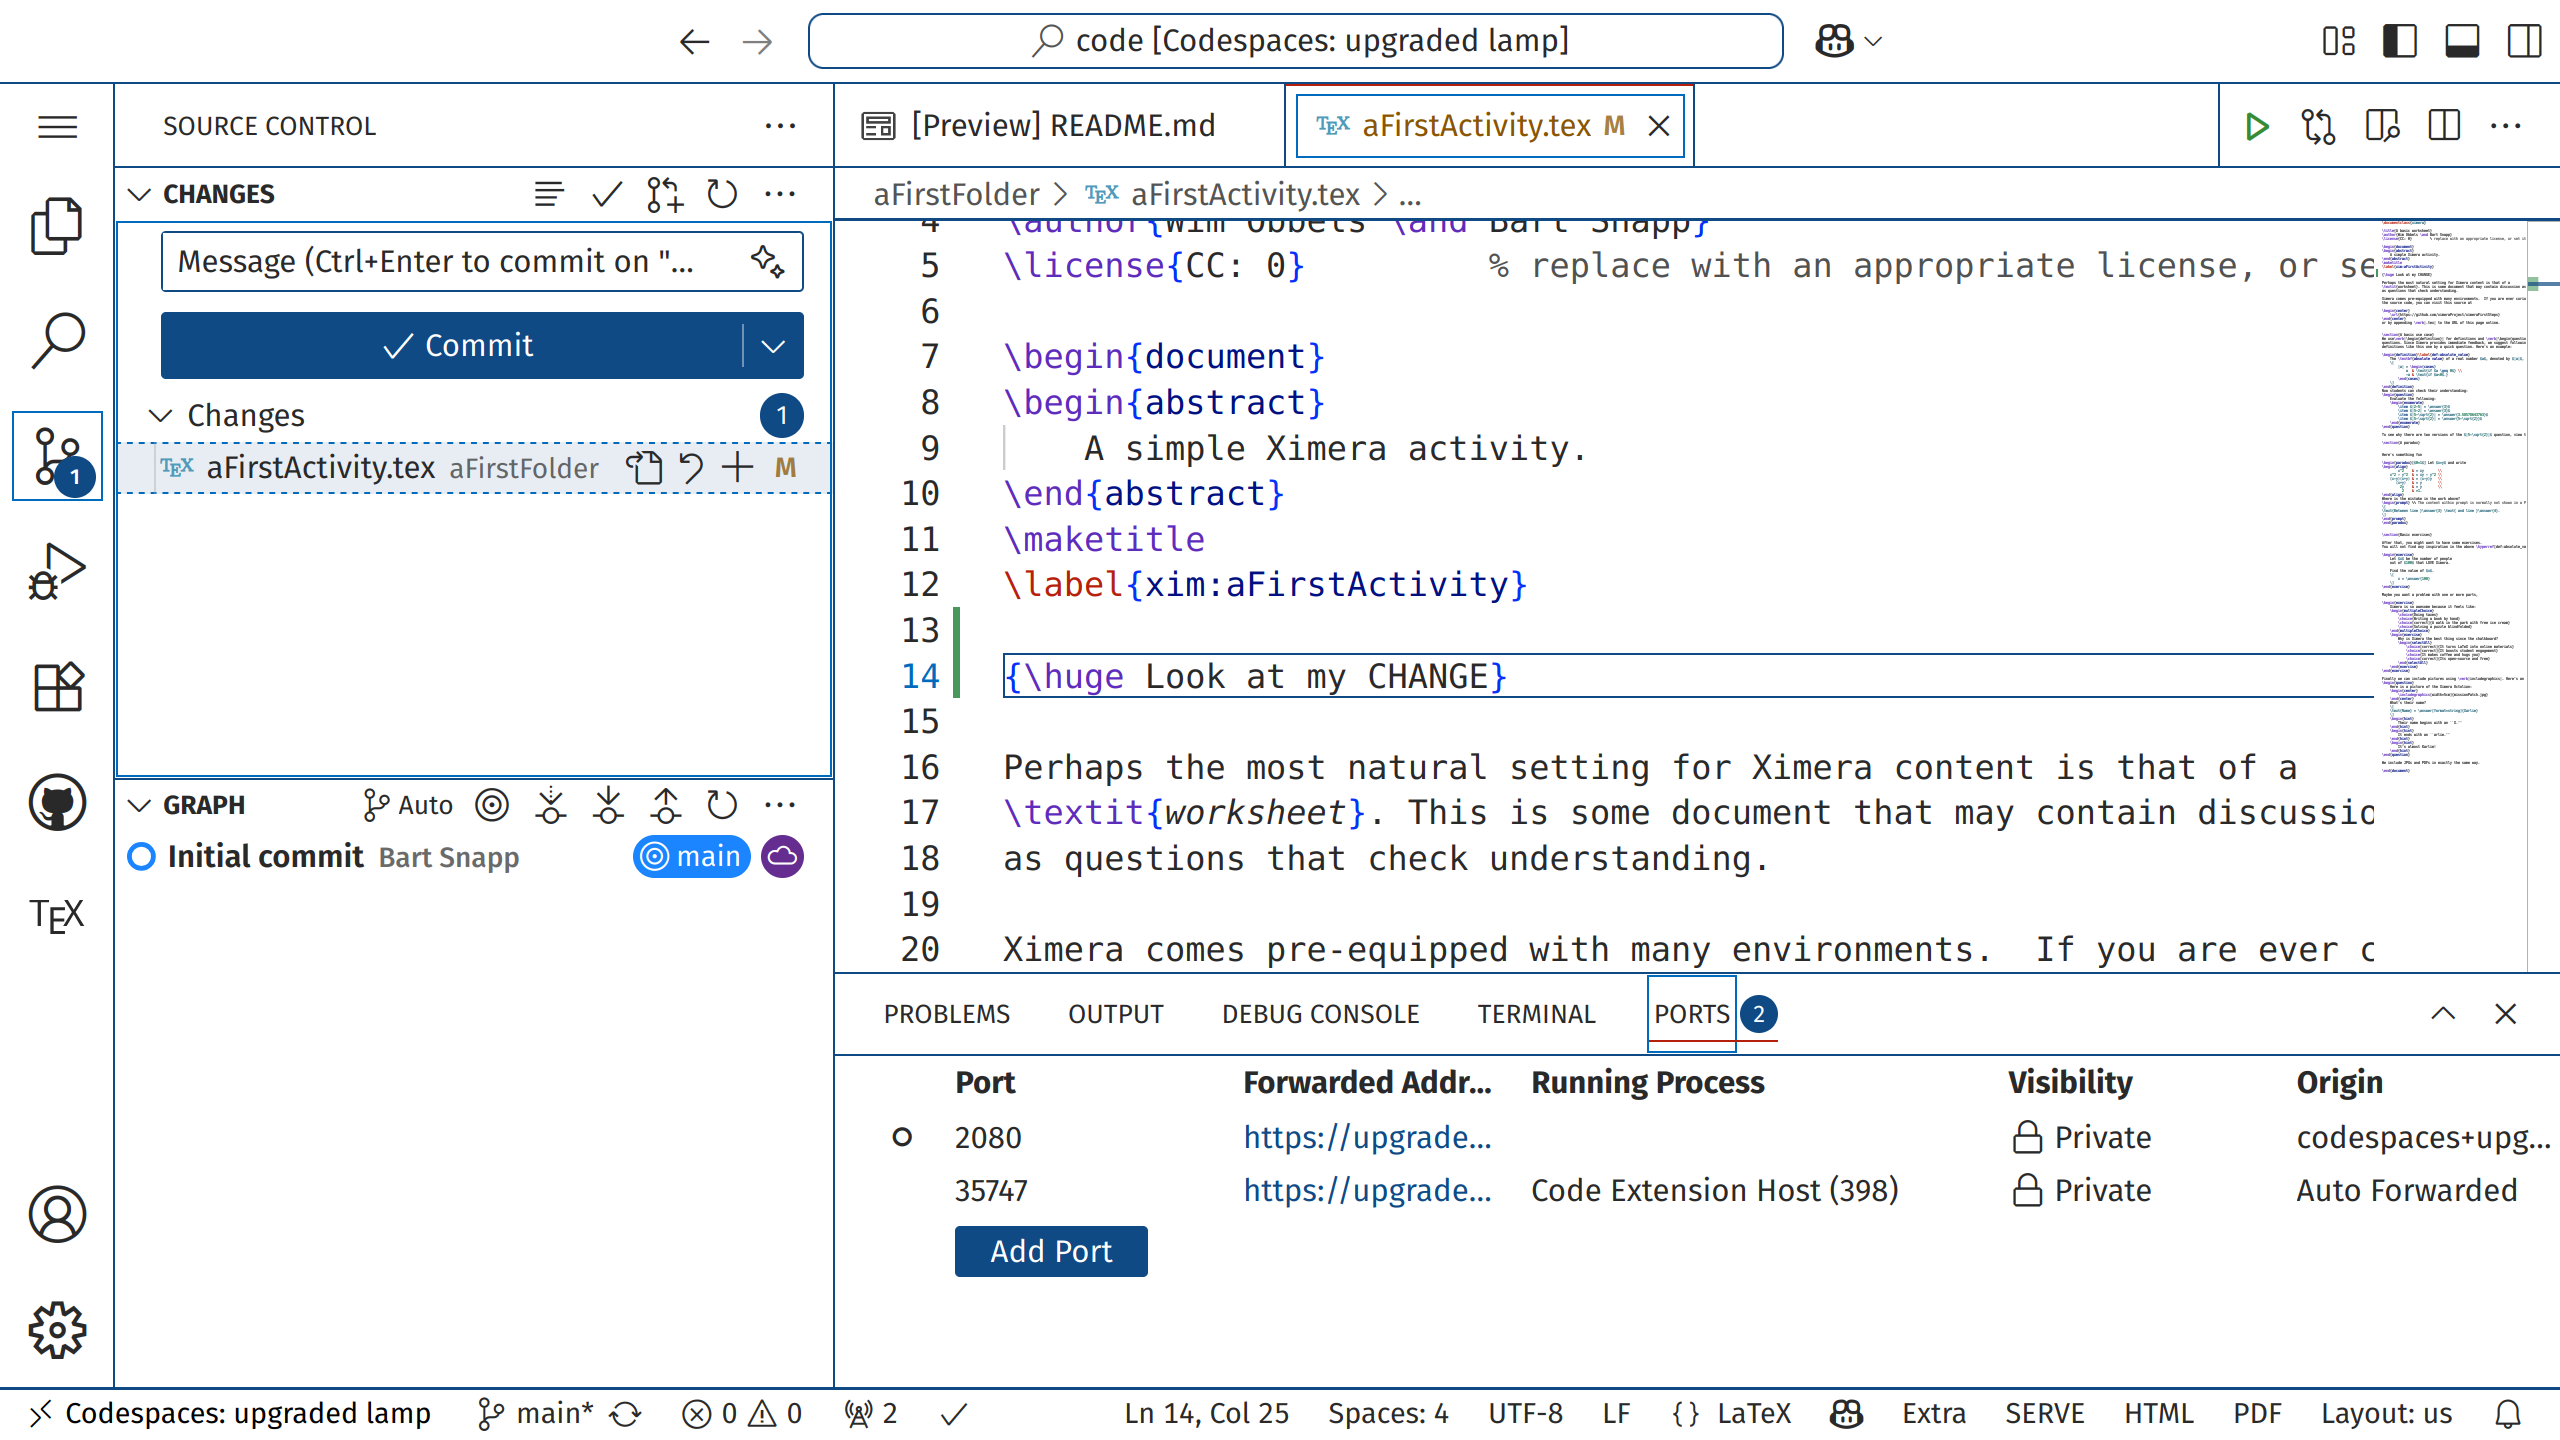
\includegraphics[width=.7\textwidth]{xfsStage}
\end{image}

\pdfOnly{\begin{multicols}{2}}
    Remember, \verb!git! is version control software. This means that it is like a magical notebook that remembers every change you
    make to your
    project. It helps you go back in time if something breaks and lets you
    share
    your work with others. For this reason, it makes you do a little ``dance''
    to ensure good code hygiene.

    \paragraph{Step 1: Staging Files (The ``+'' Button)}

    You start by clicking on the icon that looks like a poorly drawn ``Y'' with
    lines and circles on the left. Then you click on a $+$ for every file you
    want
    to send to your repository.  When you click the little \textbf{``+''} next
    to a
    file, you're saying,
    \begin{quote}
        \emph{``Hey git, this file is ready to be saved!''}
    \end{quote}

    This adds the file to a special list called the \textbf{staging area}. Only
    files in this list will be saved in the next step.

\pdfOnly{\end{multicols}}

\newpage

\begin{image}
    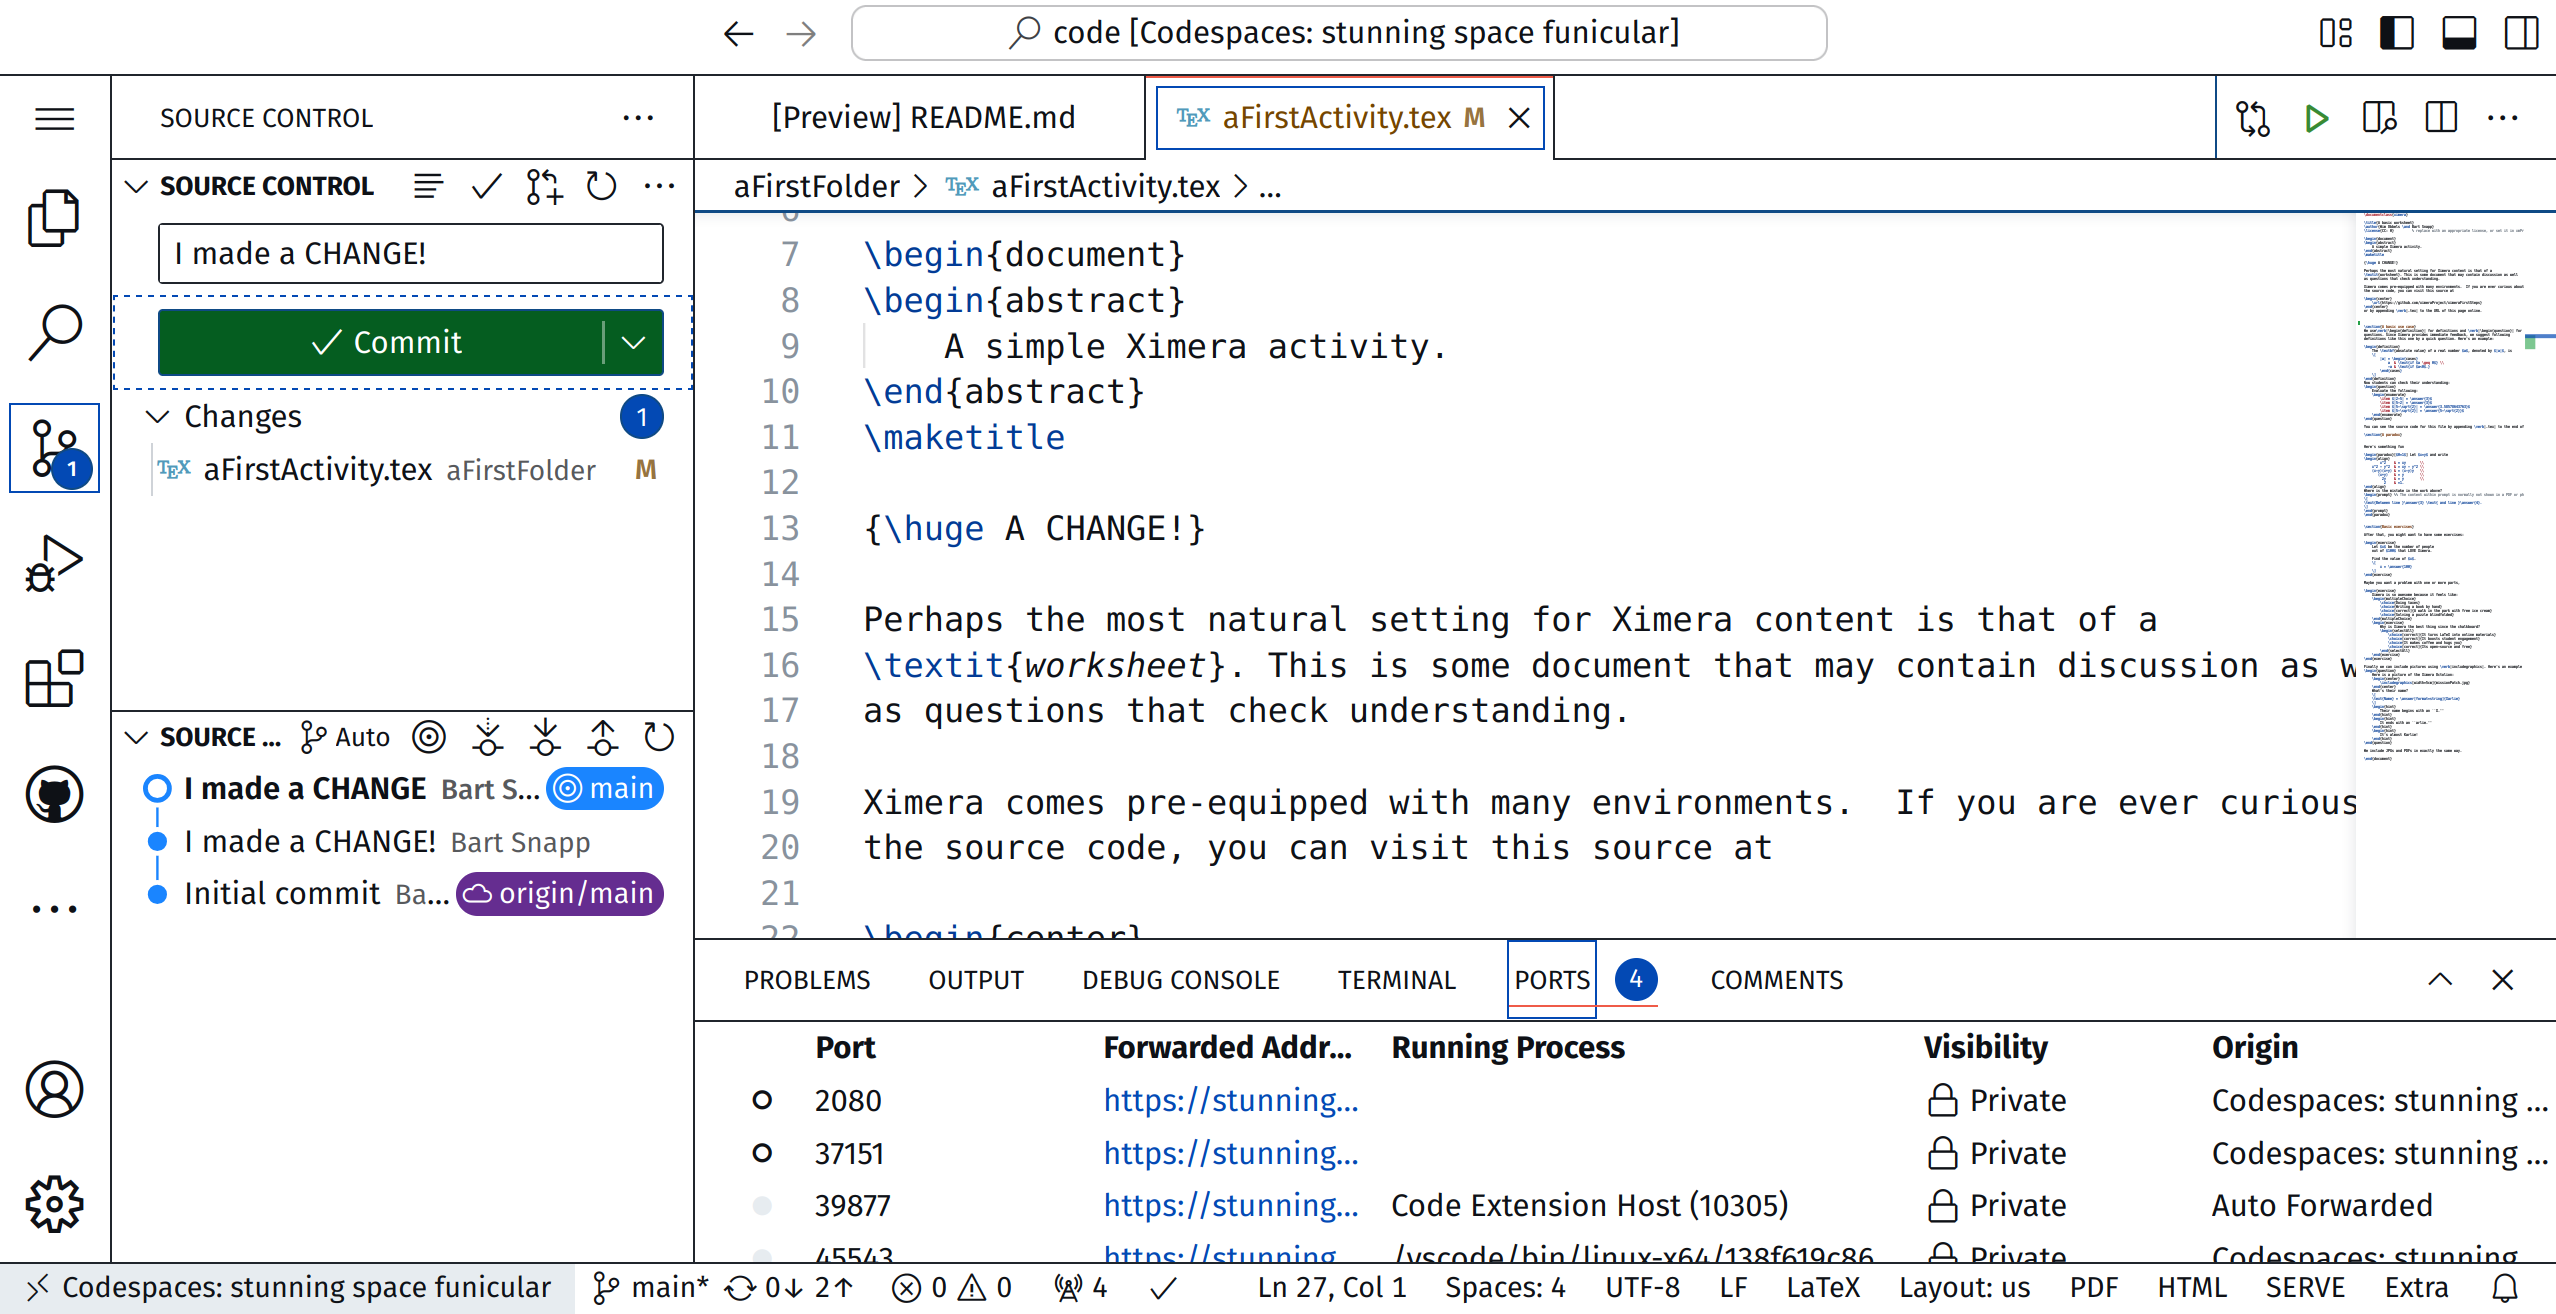
\includegraphics[width=.7\textwidth]{xfsCommitMessage}
\end{image}
\pdfOnly{\begin{multicols}{2}}
    \paragraph{Step 2: Committing Changes (Saving Your Work)}

    After staging your files, you
    \begin{enumerate}
        \item \textbf{type a message} directly above the green ``Commit''
              button.
        \item Click ``Commit.''
    \end{enumerate}
    This tells \verb!git!:
    \begin{quote}
        \emph{``Save these changes forever, and here's a note about what I
            did.''}
    \end{quote}
    \verb!git! takes a snapshot of the staged files and saves them with your message.
    If you would ever need to undo your work from this point, this message will
    help guide your future-self.
\pdfOnly{\end{multicols}}

\newpage

\begin{image}
    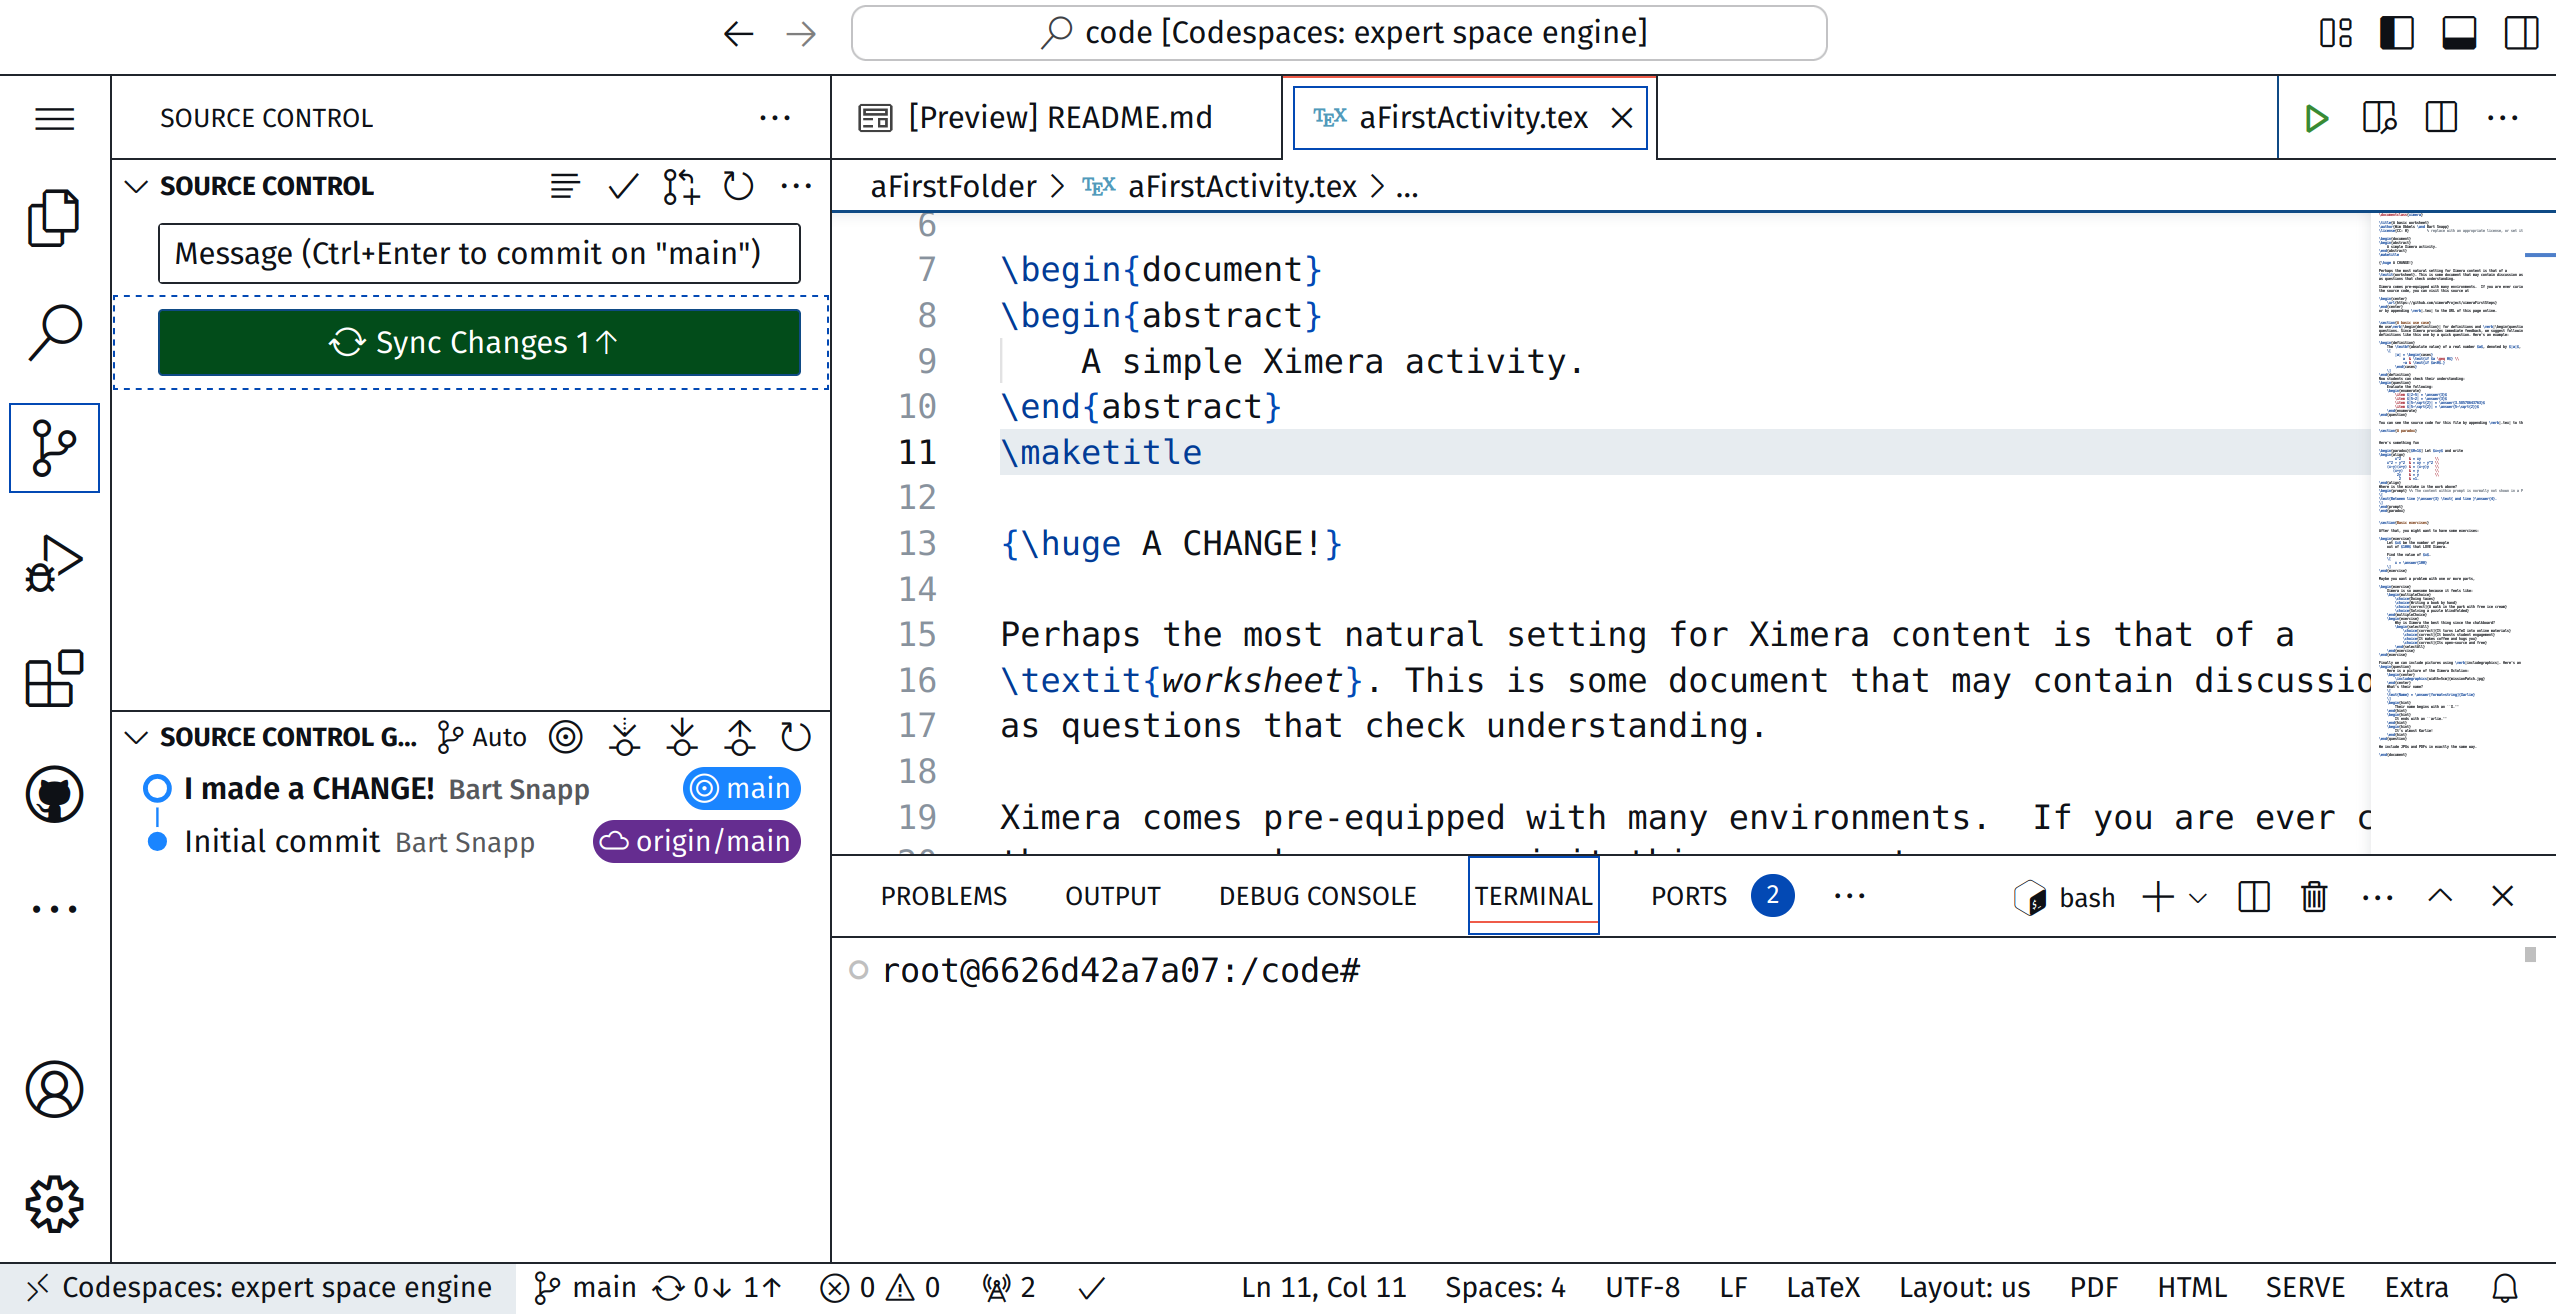
\includegraphics[width=.7\textwidth]{xfsSync}
\end{image}
\pdfOnly{\begin{multicols}{2}}
\paragraph{Step 3: Syncing with GitHub (Sending Your Work Online)}
When you click \textbf{``Sync Changes''}, you're telling \verb!git!:
\begin{quote}
    \emph{``Send my saved changes to the repository on GitHub.''}
\end{quote}
\verb!git! takes your saved changes and sends them to your \textbf{remote
    repository}
(the one on GitHub). At the same time, it checks if there are any new
changes from your teammates and brings them back to you. At this point,
VS Code in your codespace will ask you if you periodically want to sync.
You can click ``Yes.''
\pdfOnly{\end{multicols}}

\newpage

\begin{image}
    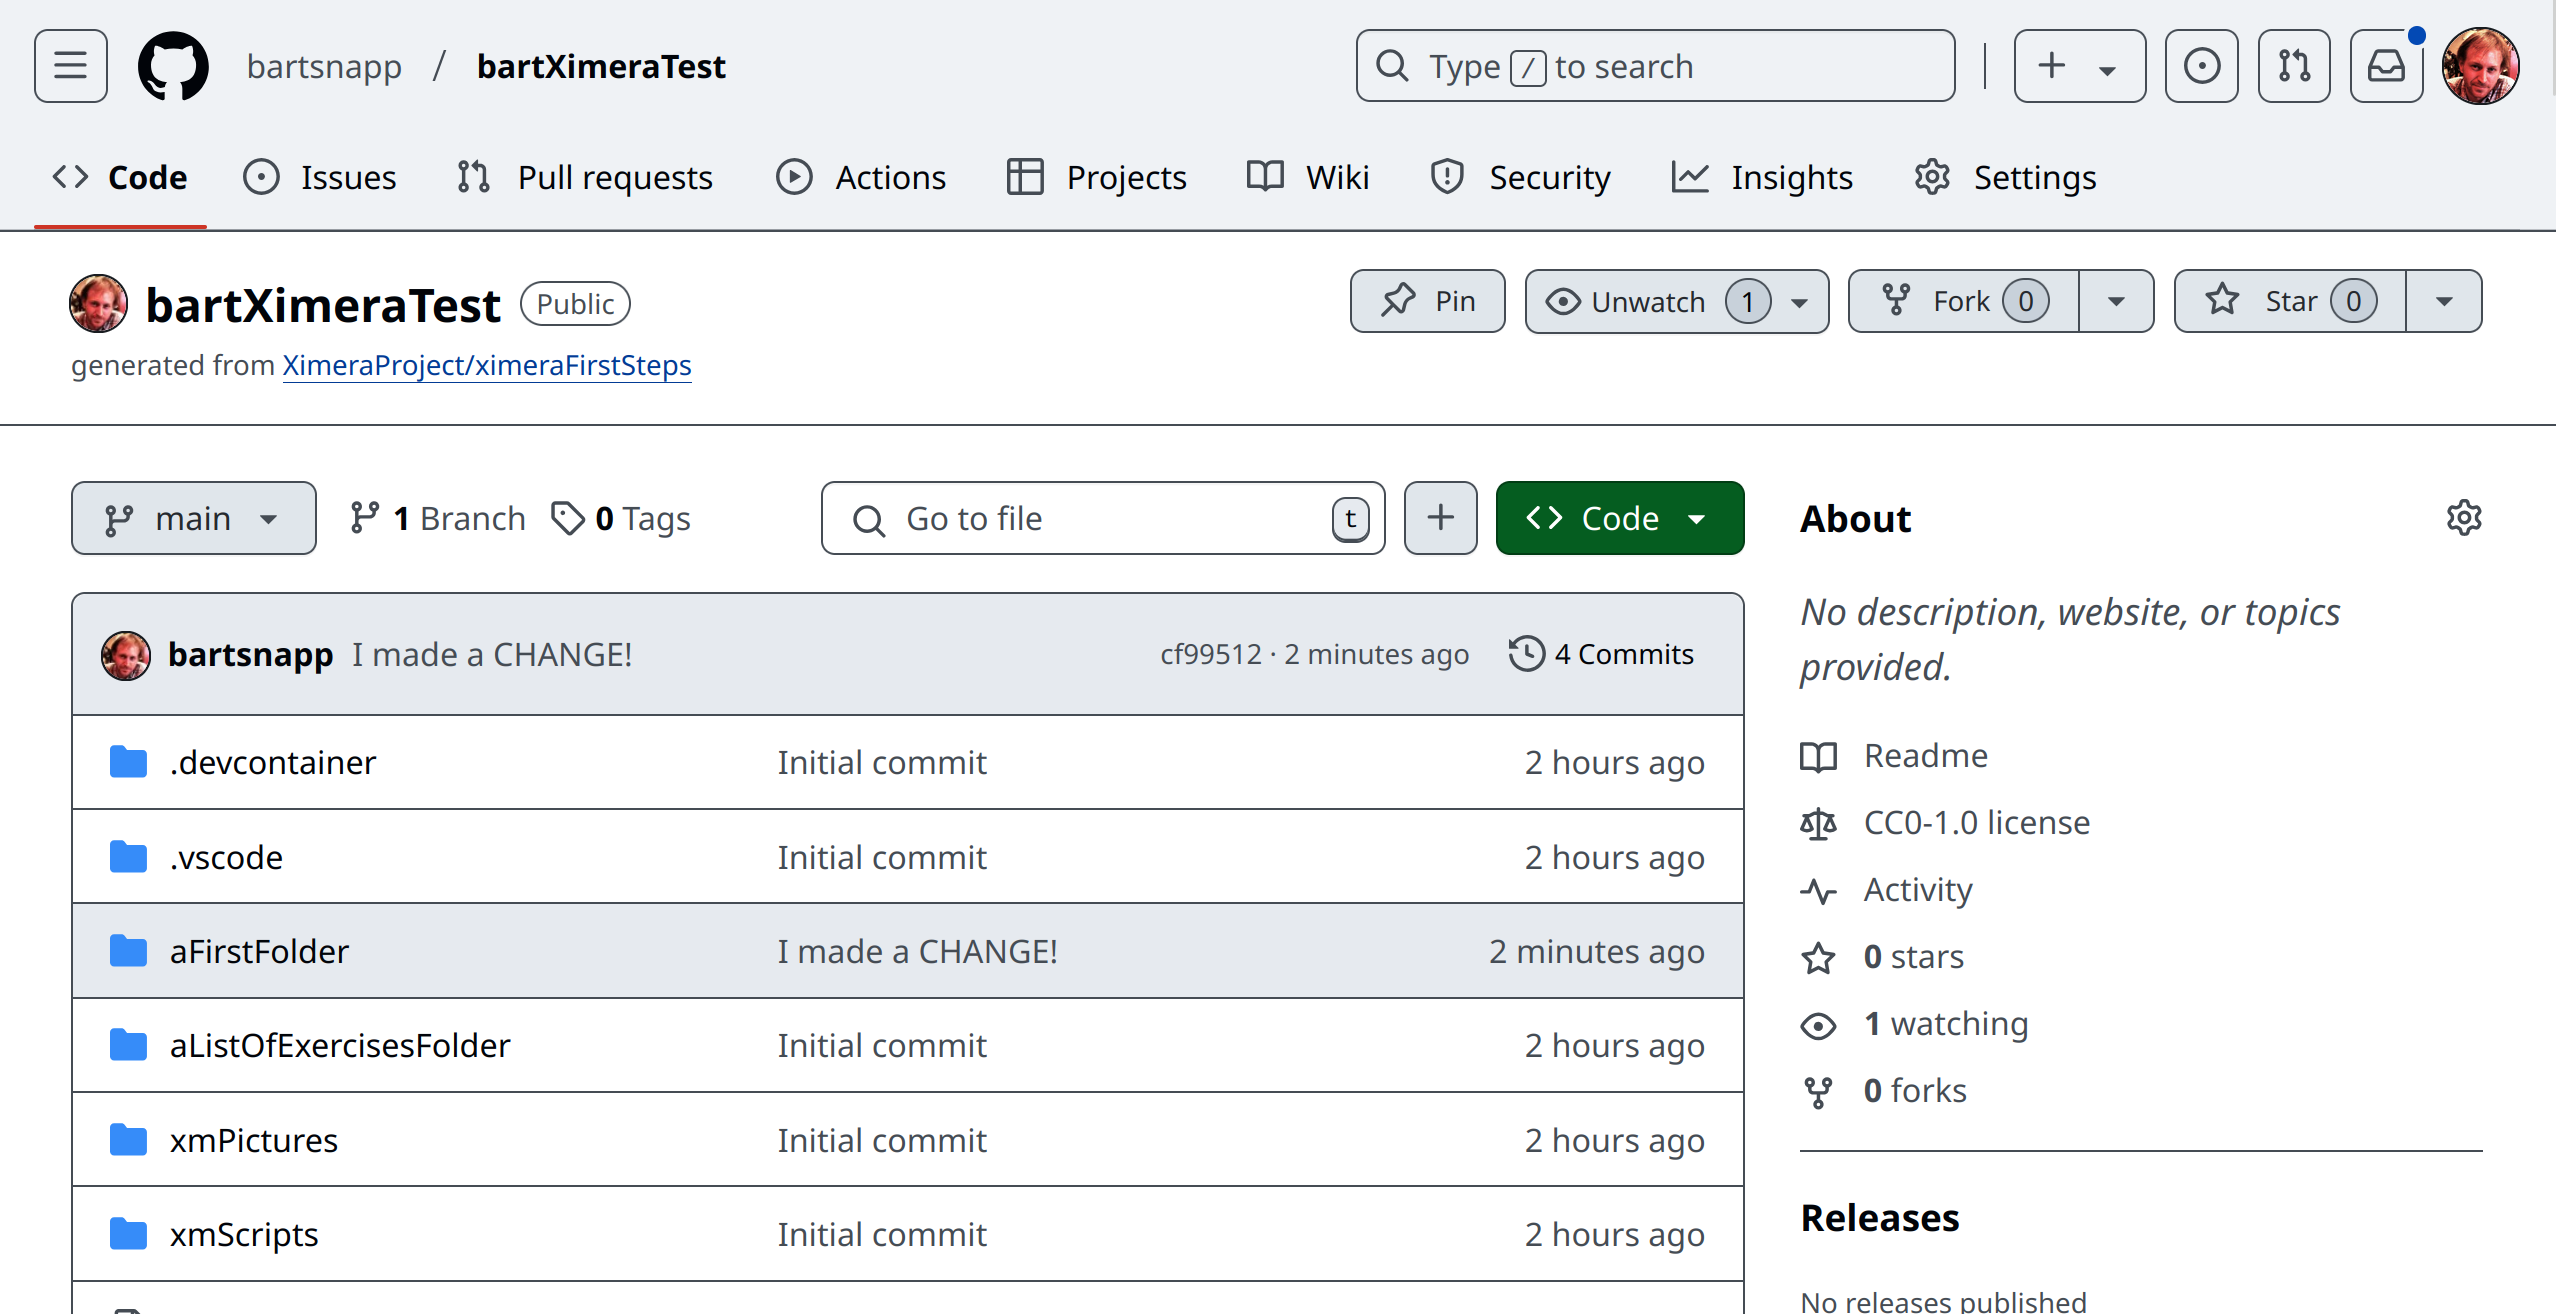
\includegraphics[width=.7\textwidth]{xfsConfirm}
\end{image}
\pdfOnly{\begin{multicols}{2}}
To check that everything worked correctly, go to
\begin{center}
    \url{https://github.com/YOUR-GIT-USER-NAME/YOUR-REPO-NAME}
\end{center}
Above we see my repository, and we see that my change was indeed made.


\paragraph{The \texttt{git} workflow} can seem overwhelming. Use the VSCode buttons, or type explicit commands in the Terminal.
\begin{description}
    \item[Stage] Select with the ``+'' button what you want to
        commit (save). Or type
{\footnotesize
\begin{verbatim}
git add FILE-NAME-1 FILE-NAME-2  # You can list multiple files or
git add -u                       # Add all modified files 
\end{verbatim}
}
    \item[Commit] Write a message and click ``Commit'' to save
          your changes. 
\begin{verbatim}
git commit -m 'A GOOD MESSAGE'
\end{verbatim}
\pdfOnly{\end{description}}
\pdfOnly{\begin{minipage}{\columnwidth}}
\pdfOnly{\begin{description}}    
    \item[Sync changes] Send your changes to GitHub and get updates from
          your  team.
\begin{verbatim}
git pull && git push
\end{verbatim}
\end{description}
\paragraph{Check} on GitHub by visiting:
\begin{center}
    \verb!https://github.com/YOUR-GIT-USER-NAME/YOUR-REPO-NAME!
\end{center}
\pdfOnly{\end{minipage}}
\pdfOnly{\end{multicols}}



\twocolumn
\end{document}